% --------------------------------------------------------------------------- %
% Poster for RC28 in Budapest         
% --------------------------------------------------------------------------- %
% Created with Brian Amberg's LaTeX Poster Template. Please refer for the     %
% attached README.md file for the details how to compile with `pdflatex`.     %
% --------------------------------------------------------------------------- %

\documentclass[a0paper,portrait]{baposter}

\usepackage{relsize}    % For \smaller
\usepackage{url}    	% For \url
\usepackage{epstopdf}	% Included EPS files automatically converted to PDF to include with pdflatex
\usepackage[T1]{fontenc}
%\usepackage{tikz}
\usetikzlibrary{decorations.pathmorphing}
\usepackage{wrapfig}
%\-usepackage{adjustbox}
 \usepackage[utf8]{inputenc}
 \usepackage{enumitem}
 \usepackage{dcolumn}
 
\renewcommand*\familydefault{\sfdefault} %% Only if the base font of the document is to be sans serif
%%% Global Settings %%%%%%%%%%%%%%%%%%%%%%%%%%%%%%%%%%%%%%%%%%%%%%%%%%%%%%%%%%%

\graphicspath{{pix/}}	% Root directory of the pictures
\tracingstats=2			% Enabled LaTeX logging with conditionals
\linespread{1}
%%% Color Definitions %%%%%%%%%%%%%%%%%%%%%%%%%%%%%%%%%%%%%%%%%%%%%%%%%%%%%%%%%

%\definecolor{bordercol}{RGB}{40,40,40}
%\definecolor{headercol1}{RGB}{186,215,230}
%\definecolor{headercol2}{RGB}{80,80,80}
%\definecolor{headerfontcol}{RGB}{0,0,0}
%\definecolor{boxcolor}{RGB}{186,215,230}
%\definecolor{bordercol}{RGB}{255,0,0} \usepackage[utf8]{inputenc}
%\definecolor{headercol1}{RGB}{0,255,0}
%\definecolor{headercol2}{RGB}{0,0,255}
\definecolor{headerfontcol}{RGB}{20,20,20}
\definecolor{boxcolor}{RGB}{255,255,0}
\definecolor{dunkelblau}{RGB}{0,58,90}
\definecolor{mittelblau}{RGB}{160,201,232}
\definecolor{hellblau}{RGB}{211,228,244}
\definecolor{hellgrau}{RGB}{220,221,221}
\definecolor{mittelgrau}{RGB}{183,184,186}
\definecolor{dunkelgrau}{RGB}{116,115,118}
\definecolor{rot}{RGB}{226,0,60}
\definecolor{fastweiss}{RGB}{240,240,240}
\definecolor{schwarz}{RGB}{0,0,0}

%%%%%%%%%%%%%%%%%%%%%%%%%%%%%%%%%%%%%%%%%%%%%%%%%%%%%%%%%%%%%%%%%%%%%%%%%%%%%%%%
%%% Utility functions %%%%%%%%%%%%%%%%%%%%%%%%%%%%%%%%%%%%%%%%%%%%%%%%%%%%%%%%%%

%%% Save space in lists. Use this after the opening of the list %%%%%%%%%%%%%%%%
\newcommand{\compresslist}{
	\setlength{\itemsep}{1pt}
	\setlength{\parskip}{0pt}
	\setlength{\parsep}{0pt}
}

%%%%%%%%%%%%%%%%%%%%%%%%%%%%%%%%%%%%%%%%%%%%%%%%%%%%%%%%%%%%%%%%%%%%%%%%%%%%%%%
%%% Document Start %%%%%%%%%%%%%%%%%%%%%%%%%%%%%%%%%%%%%%%%%%%%%%%%%%%%%%%%%%%%
%%%%%%%%%%%%%%%%%%%%%%%%%%%%%%%%%%%%%%%%%%%%%%%%%%%%%%%%%%%%%%%%%%%%%%%%%%%%%%%

\begin{document}

\typeout{Poster rendering started}

%%% Setting Background Image %%%%%%%%%%%%%%%%%%%%%%%%%%%%%%%%%%%%%%%%%%%%%%%%%%
%\background{

%	\begin{tikzpicture}[remember picture,overlay]%
%	\draw (current page.north west)+(-2em,2em) node[anchor=north west]
%	{\includegraphics[height=1.1\textheight]{background}};
%	\end{tikzpicture}
%}

%%% General Poster Settings %%%%%%%%%%%%%%%%%%%%%%%%%%%%%%%%%%%%%%%%%%%%%%%%%%%
%%%%%% Eye Catcher, Title, Authors and University Images %%%%%%%%%%%%%%%%%%%%%%
\begin{poster}{
	grid=false,
	% Option is left on true though the eyecatcher is not used. The reason is
	% that we have a bit nicer looking title and author formatting in the headercol
	% this way
	eyecatcher=true,
	borderColor=dunkelgrau,
	%headerColorOne=mittelblau,
	headerColorOne=schwarz,
	%headerColorTwo=mittelblau,
	headerColorTwo=schwarz,
	headerFontColor=fastweiss,
	% Only simple background color used, no shading, so boxColorTwo isn't necessary
	%boxColorOne=hellblau,
	boxColorOne=fastweiss,
	headershape=rectangle,
	headerfont=\Large\sf\bf,
	textborder=rectangle,
	background=none,
	%bgColorOne=hellblau,
	bgColorOne=hellgrau,
	headerborder=closed,
	%headershade=shade-lr,
	linewidth=0.2,
  boxshade=plain
}
%%% Eye Cacther %%%%%%%%%%%%%%%%%%%%%%%%%%%%%%%%%%%%%%%%%%%%%%%%%%%%%%%%%%%%%%%
{
	%Eye Catcher, empty if option eyecatcher=false - unused
	%
\includegraphics[width=12em]{Universitaet_Bern.pdf}
}
%%% Title %%%%%%%%%%%%%%%%%%%%%%%%%%%%%%%%%%%%%%%%%%%%%%%%%%%%%%%%%%%%%%%%%%%%%
{\sf\bf\huge
	Inequality of income in Switzerland
}
%%% Authors %%%%%%%%%%%%%%%%%%%%%%%%%%%%%%%%%%%%%%%%%%%%%%%%%%%%%%%%%%%%%%%%%%%
{
	\vspace{1em}Rudolf Farys (Uni Bern), Oliver Hümbelin (BFH)
  %{\smaller \texttt{oliver.huembelin@bfh.ch}}
  %\vspace{1em} Rudolf Farys\\
  %{\smaller \texttt{rudolf.farys@soz.unibe.ch}}
}
%%% Logo %%%%%%%%%%%%%%%%%%%%%%%%%%%%%%%%%%%%%%%%%%%%%%%%%%%%%%%%%%%%%%%%%%%%%%
{
% The logos are compressed a bit into a simple box to make them smaller on the result
% (Wasn't able to find any bigger of them.)


\includegraphics[height=10em]{Universitaet_Bern.pdf}

\includegraphics[height=8em]{BFH_Logo_A_de_100_4CU.eps}

}


\headerbox{Summary}{name=summary,column=0,row=0}{
We outline recent developments in Switzerland regarding income and income inequality using data on an individual and community level. We find ... You can find more information and visualizations at our project website: \texttt{http://inequalities.ch}.
}

\headerbox{Data}{name=data,column=1,row=0}{
We use two different data sets. On a community level our data are provided by the Swiss Federal Tax Administration. Individual data were collected with the help of the cantonal tax administrations of Aargau and Obwalden. Our variable of interest is inequality of income: a Gini coefficient we derive from \texttt{taxable income} which is the sum of all sorts of income (wages, dividends, rent, etc.) minus all possible deductions. 
}

\headerbox{Unified Theory}{name=ut,column=0,span=2,below=data}{
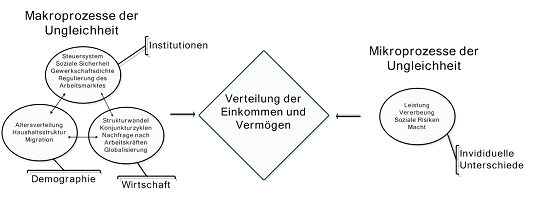
\includegraphics[width=\textwidth]{../figure/ut}
}

\headerbox{Descriptives}{name=descriptives,column=0,below=ut,span=2}{
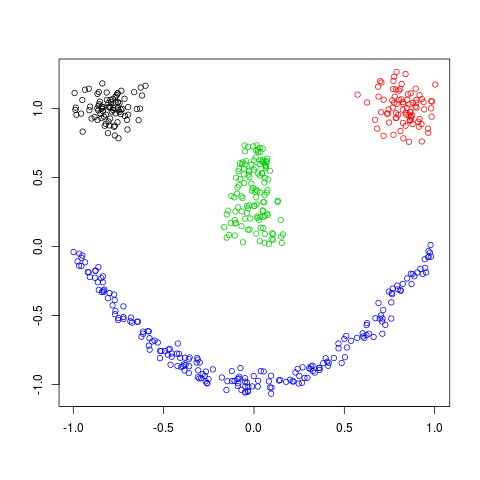
\includegraphics[width=0.5\textwidth]{../figure/smiley}
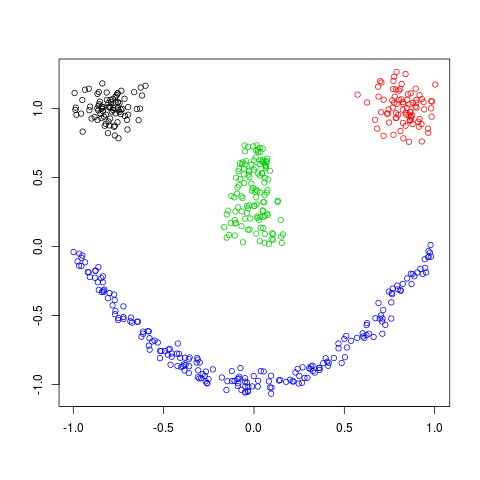
\includegraphics[width=0.5\textwidth]{../figure/smiley}
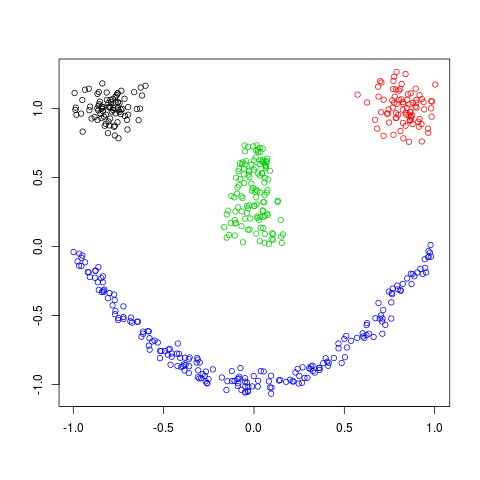
\includegraphics[width=0.5\textwidth]{../figure/smiley}
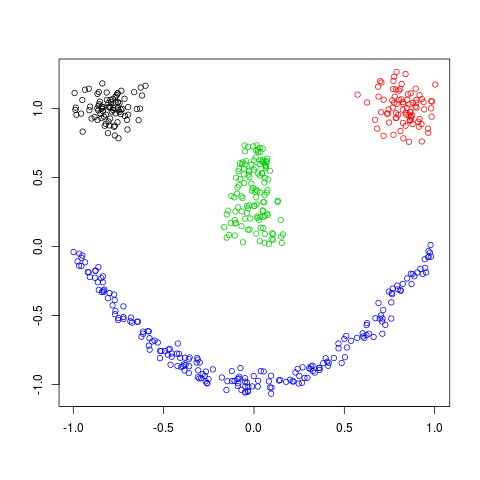
\includegraphics[width=0.5\textwidth]{../figure/smiley}
}

\headerbox{Discussion/Results}{name=results,column=2,span=1,row=0}{
\begin{itemize}[leftmargin=12pt]
\item On the community level we see support for H1, H2, H4 but not for H3. H5, H6 and H7 are only testable with individual data.
\item On an individual level we find support for H5 and H6 but not H7.
\end{itemize}

Bla bla bla Bla bla bla Bla bla bla Bla bla bla Bla bla bla Bla bla bla 
}


\headerbox{Regression Analyses}{name=model,column=2,span=1,below=results}{
\centerline{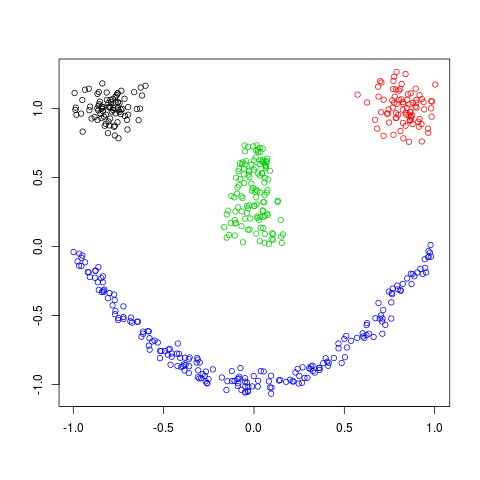
\includegraphics[width=\textwidth]{../figure/smiley}}
\begin{tabular}{ l D{.}{.}{2}D{.}{.}{2} } 
\hline 
  & \multicolumn{ 1 }{ c }{ Model 1 } & \multicolumn{ 1 }{ c }{ Model 2 } \\ \hline
 %          & Model 1 & Model 2\\ 
groupTrt   & 4.66 ^* & -0.37  \\ 
           & (0.22)  & (0.31)  \\
 $N$        & 20      & 20     \\ 
$R^2$      & 0.98    & 0.07   \\ 
adj. $R^2$ & 0.98    & 0.02   \\ 
Resid. sd  & 0.70    & 0.70    \\ \hline
 \multicolumn{3}{l}{\footnotesize{Standard errors in parentheses}}\\
\multicolumn{3}{l}{\footnotesize{$^*$ indicates significance at $p< 0.05 $}} 
\end{tabular} 

Bla bla bla Bla bla bla Bla bla bla Bla bla bla Bla bla bla Bla bla bla 
}



\end{poster}
\end{document}


